\include{SupportVectorMachinesAndFlexibleDiscriminants}
\section{Support Vector Machines and Flexible Discriminants}
The optimal separating hyperplane separates the two classes and maximizes the distance to the closest point from either class (Vapnik, 1996). Not only does this provide a unique solution to the separating hyperplane problem, but by maximizing the margin between the two classes on the training data, this leads to better classification performance on test data.
\iffalse
Suppose $M$ is the distance. Then

\begin{equation}
\begin{aligned}
&\max\limits_{\beta,\beta_0, ||\beta||=1} M \\
& y_i(x_i^T\beta + \beta_0) \ge M
\end{aligned}
\end{equation}

We  can move the constrain on the module $\||\be||=1$ to the condition $\frac{1}{||\be||}y_i(x_i^T\beta + \beta_0) \ge M$, which redefines $\be_0$. 

For a pair of coefficients satisfying this inequalities, any positively scaled multiple satisfies them too, so we can set arbitrarily set $||\be||=\frac{1}{M}$:

\begin{equation}
\begin{aligned}
&\min_{\be, \be_0}{\frac{1}{2}||\be||^2}\\
\textit{subject to } &y_i(x_i^T\be+\be_0)\ge1
\end{aligned}
\end{equation}

With this constraint, a margin around the decision boundary with thick $\frac{1}{||\be||}$ is present. We choose $\be$ to maximize the thickness of margin margin.  This is a convex optimization problem. The Lagrange primal function to be minimized is:

\begin{equation}
\label{eq}
L_p = \frac{1}{2} ||\be||^2 = \sum_{i=1}^N \alpha_i\left[ y_i \br{x_i^T\be+\be_0}\right]

\end{equation}

and setting the derivatives to $0$:

\begin{equation}
\begin{aligned}
\be &= \sum_{i=1}^N \alpha_i y_i x_i
0  &= \sum_{i=1}^N \alpha_i y_i
\end{aligned}
\end{equation}

and substituting in \autoref{eq}:

\begin{equation}
\begin{aligned}
L_D = \sum_{i=1}^N \alpha_i -\frac{1}{2}\sum_{i=1}^N\sum_{k=1}^N \alpha_i \alpha_ky_iy_kx_i^Tx_k\\
\textit{subject to } \alpha_i\ge0 \textit{ and } \sum_{i=1}^N \alpha_iy_i=0
\end{aligned}
\end{equation}
\fi

The optimal hyperplane (or hard margin SVM) focuses more on points that counts, i.e., close to the border, that are called \tb{support vector}. For this reason it is more robust. LDA depends on all the data, even points faraway. If classes are really Gaussian LDA is optimal and separating hyperplane will pay a price for focusing on noisier data.
For logistic regression, if a separate hyperplane exists, since the log-likelihood can be driven to $0$.

When data are not separable there will be no feasible solution and an alternative formulation is needed. In this case the we allow some points to be beyond the margin and the problem is generally referred to as \ti{soft margin classification}.

First we analyze the hard margin SVM classification problem with the following steps, then extend it to the non perfectly separable case with the soft margin classification and finally show how it can work for regression as well.

\subsection{Hard margin Support Vector Machine classification}
\label{HardMarginSVM}
\textit{https://nlp.stanford.edu/IR-book/html/htmledition/support-vector-machines-the-linearly-separable-case-1.html}
\textit{https://www.youtube.com/watch?v=\_PwhiWxHK8o}

We will follow the following steps:

\begin{figure}
\centering
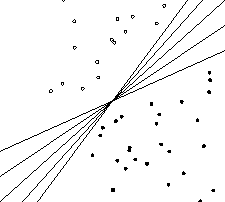
\includegraphics[scale=0.6]{img/separableClasses}
\caption{Example of infinite lines separating two perfectly separable classes.}
\label{separableClasses}
\end{figure}

Consider two classes on a space (for example a two dimensional space as in \autoref{separableClasses}) and suppose the two classes are perfectly separable. We want to divide the two classes with a straight line. The problem becomes to define what is the best straight line since such lines exist. The solution is to choose the line that separates the classes as much as possible, lying as faraway as possible from both the classes. Such line can be thought as the middle line of a street separating the two classes; then we want to fit the widest possible street between the two classes (see \autoref{separableClassesPy}). The closest occurrences of the two classes closest to the separator defines the margins, the gutters of the street (the dashed lines in \autoref{separableClassesPy}).

\begin{figure}
\centering
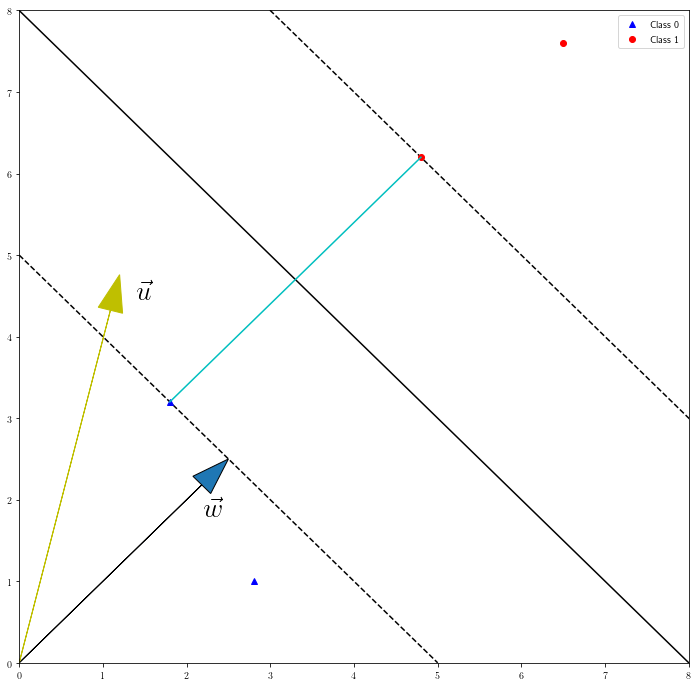
\includegraphics[scale=0.4]{img/separableClassesPy}
\caption{Example of best separating line maximizing the margin.}
\label{separableClassesPy}
\end{figure}

Let us consider a vector $\vec{w}$ of any length, perpendicular to the gutters of the street and consider an unknown instance to be classified (\autoref{separableClassesPy}) called $\vec{u}$. To see if this unknown is on the left or right side of the street, we project its vector $\vec{u}$ onto the vector $\vec{w}$ that is perpendicular to the street. The bigger this product, the more likely the point is to be on the right side of street, hence the more likely it is to be of class $+$.

Mathematically:
\begin{equation}
\vec{u}\cdot \vec{w} \ge c \Leftrightarrow \vec{u}\cdot \vec{w} + b \ge0\Rightarrow \text{Class } 1 \quad\quad \text{with } b=-c
\end{equation}
This is the \tb{decision rule}. The problem is that both $\vec{w}$ and $b$ are unknown; only the direction of $\vec{w}$ is known but not its length.

\tb{Other constraints must be added} to calculate $\vec{w}$ and $b$. Now suppose one positive and one negative instances $x_+$ and $x_-$ are given. We want:
\begin{equation}
\begin{aligned}
\vec{w} \cdot \vec{x}_+ + b &\ge 1\\
\vec{w} \cdot \vec{x}_- + b &\le -1
\end{aligned}
\end{equation}
Just for mathematical convenience we introduce a new variable $y_i$ for each instance such that:
\begin{equation}
\begin{aligned}
y_i = 1 \quad \text{if } \vec{x}_+\\
y_i = -1 \quad \text{if } \vec{x}_-\\ 
\end{aligned}
\end{equation}
In this way:
\begin{equation}
y_i (\vec{w}\cdot \vec{x}_i + b) \ge 1
\end{equation}
that can be rearranged as:
\begin{equation}
y_i (\vec{w}\cdot \vec{x}_i + b) -1 \ge 0
\end{equation}

Now \tb{another constraint} is going to be added: \tb{the previous equation is forced to be $0$ for the points in the gutter}, i.e., on the margins:
\begin{equation}
y_i (\vec{w}\cdot \vec{x}_i + b) -1 = 0
\label{SVMmargin}
\end{equation}

\begin{figure}
\centering
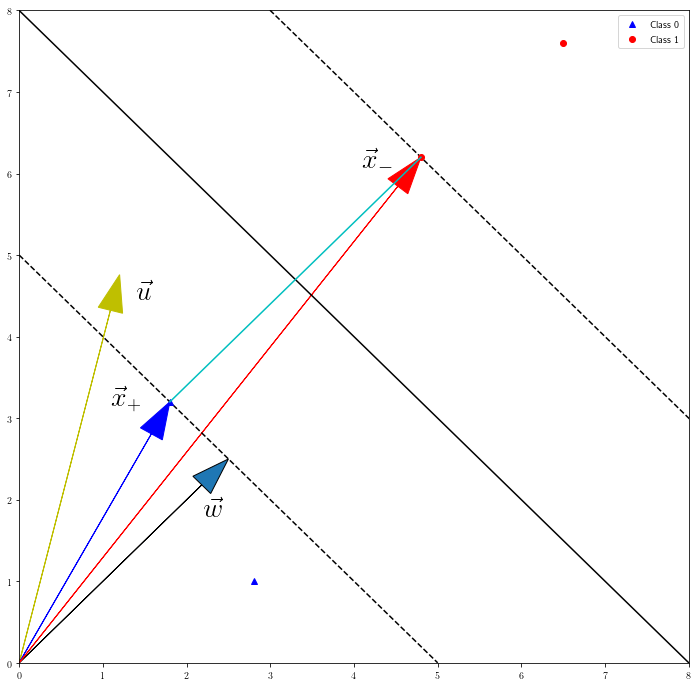
\includegraphics[scale=0.4]{img/SVMwidth}
\caption{Derivation of the width.}
\label{SVMwidth}
\end{figure}

So this equation holds for the points $x_+$ and $x_-$ that are closest to the separator (the black solid line on the previous plots), i.e., the ones that decide and limit the width of the street. Now we need to express the width of the street. Consider the difference between these two points $(\vec{x}_+ - \vec{x}_-)$ (\autoref{SVMwidth}) and project it onto the normal: \textbf{this is exactly the width of the street}.
\begin{equation}
\begin{aligned}
\text{width} = 2M = \left( \vec{x}_+ - \vec{x}_-\right) \cdot \frac{\vec{w}}{\norm{\vec{w}}}
\end{aligned}
\label{width0}
\end{equation}

For $\vec{x}_+$, $y_i=1$. From \autoref{SVMmargin}:
\begin{equation}
\vec{w} \vec{x}_+ + b = 1\Rightarrow \vec{w} \vec{x}_+ = 1-b
\end{equation}
for the same reason, considering $x_-$:
\begin{equation}
-\vec{w} \vec{x}_- - b = 1\Rightarrow -\vec{w} \vec{x}_+ = 1+b
\end{equation}

So substituting in \autoref{width0}:
\begin{equation}
\begin{aligned}
\text{width} = \frac{2}{\norm{\vec{w}}}
\end{aligned}
\label{width1}
\end{equation}

\tb{Now we have to maximize the width}:
\begin{equation}
\max \frac{2}{\norm{\vec{w}}} \Leftrightarrow \max \frac{1}{\norm{\vec{w}}} \Leftrightarrow\min \norm{\vec{w}} \Leftrightarrow \min \frac{1}{2} \norm{\vec{w}}^2
\label{SVMmin}
\end{equation}

We have the expression \autoref{SVMmin} for which we want to find the minimum, its extreme, and we have the constraint \autoref{SVMmargin}. By \tb{Lagrange}, if we want to find the extreme of a function with constraints, then we have to use \tb{Lagrange multipliers} which will result in a new expression that can be maximized or minimized directly without any constraint. 
\begin{equation}
L(\vec{w}, b) = \frac{1}{2}\norm{\vec{w}}^2 - \sum_i \alpha_i\left[ y_i\left( \vec{w}\cdot \vec{x}_i+b\right)-1\right]
\label{SVMLagranceMult}
\end{equation}
where the second term is a sum of all the constraints weighted by $\alpha_i$, the Lagrange multipliers. These multipliers will be different from $0$ for only the points in the gutter; if the same class has more than one point on the margin then all of them will be part of the expression. We need to find the extreme of this expression. To do that, we take the derivatives and set them to $0$.
\begin{equation}
\begin{aligned}
&\frac{\partial L}{\partial \vec{w}} = w - \sum_i \alpha_i y_i \vec{x}_i = 0 \Rightarrow &\vec{w} = \sum_i \alpha_i y_i \vec{x}_i
\end{aligned}
\label{SVMLagrDevw}
\end{equation}
This tells that the vector $\vec{w}$ is a linear combination of all the sample vectors lying on the margin, the \tb{support vector}.

Differentiating with respect to $b$:
\begin{equation}
\begin{aligned}
&\frac{\partial L}{\partial b} = \sum_i \alpha_i y_i = 0 \Rightarrow \sum_i \alpha_i y_i = 0
\end{aligned}
\label{SVMLagrDevb}
\end{equation}

We try to substitute these results in \autoref{SVMLagranceMult} to find its extreme:
\begin{equation}
\begin{aligned}
L &= \frac{1}{2} \left(  \sum_i \alpha_i y_i \vec{x}_i\right) \left( \sum_j \alpha_j y_j \vec{x}_j\right) - \sum_i \alpha_i y_i \vec{x}_i \cdot\left(\sum_j \alpha_j y_j \vec{x}_j\right) -\sum_i \alpha_i y_i b + \sum_i \alpha_i =\\
& = \frac{1}{2} \left(  \sum_i \alpha_i y_i \vec{x}_i\right) \left( \sum_j \alpha_j y_j \vec{x}_j\right) - \sum_i \alpha_i y_i \vec{x}_i \cdot\left(\sum_j \alpha_j y_j \vec{x}_j\right) -b \cancel{\sum_i \alpha_i y_i} + \sum_i \alpha_i  =\\
&= \sum_i \alpha_i - \frac{1}{2}\sum_i \sum_j \alpha_i \alpha_j y_i y_j \vec{x}_i \cdot \vec{x}_j 
\end{aligned}
\end{equation}
where $b$ has been taken out of the sum since it is a constant. This expression allows to see what the value of the extreme point depends on with respect to these vectors. It depends only on the dot product of pairs of samples.

Let us see how the decision rule is affected:
\begin{equation}
\sum_i \alpha_i y_i \vec{x}_i \cdot \vec{u} + b \ge 0 \Rightarrow \vec{u} \text{ belongs to class } +
\end{equation}

Note that the space we are working on is a convex space, so there is no chance to get stuck in a local minimum/maximum, as opposite to neural nets.

This process does not work with linear inseparable problems. In these cases we can switch to another space: we call this transformation $\phi(\vec{x})$. The maximization process depends only on the dot product, so we just need to find $\phi(\vec{x}_i)\cdot \phi(\vec{x}_j)$ in order to maximize in the new space. So actually the mapping function $\phi(\cdot)$ is not needed to be known, we need to know a function such as
\begin{equation}
K(\vec{x}_i, \vec{x}_j) = \phi(\vec{x}_i)\cdot \phi(\vec{x}_j)
\end{equation} 
Such a function is called \tb{Kernel function}. Popular choices of kernels are
\begin{itemize}
\item linear kernel $\left(\vec{u} \cdot \vec{v}+1\right)^n$
\item $e^{-\frac{\norm{\vec{x}_i - \vec{x}_j}}{\sigma}}$: be careful to choose a not too small $\sigma$ the points are shrunk around and we get overfitting.
\end{itemize}

We have seen \textbf{Optimal separating hyperplabes} in \autoref{OSH}. Here we will see the case for non-separable classes, where the classes overlap.
\subsection{Soft Margin Support Vector Machine}
The hard margin SVM works well when data do not contain outliers or noisy samples close to the separator. In such cases, the outlier can make the margin too small or move the separator toward the other class and this might cause misclassification. It is generally preferable to have a fat margin allowing to some noisy samples to be inside or on the wrong side of the margin.

We still want to maximize the margins $M$ allowing some points to be on the wrong side. For each misclassified point we pay a cost proportional to its distance from the margin. To do this, we define a slack variable $\xi=\br{\xi_1, \xi_2, \cdots, \xi_N}$ with $\xi_i\ge 0$, whose value is not null for the points beyond the margin:
\begin{equation}
\xi_i = \max \left(0, 1-y_i(\vec{w}\vec{x_i}+b)\right)
\end{equation}
where $1-y_i(\vec{w}\vec{x_i}+b)$ is proportional to the distance from the margin.	
The decision rule hence becomes:
\begin{equation}
\begin{aligned}
& y_i \left( \vec{w} \vec{x}_i + b\right) \ge 1 - \xi_i \Rightarrow y_i \left( \vec{w} \vec{x}_i + b\right) - 1+ \xi_i  \ge 0 \\
& \xi_i \ge 0
\end{aligned}
\end{equation}
However, we want to limit the number of misclassified points so the objective becomes
\begin{equation}
\begin{aligned}
&\min \frac{1}{2} \norm{\vec{w}} + C \sum_i \xi_i\\
\textit{subject to }&\left\{
		\begin{array}{ll}
				y_i(\vec{w} \cdot \vec{x}_i+b) \ge 1-\xi_i\\ 
 				\xi_i \ge 0
		\end{array} 
\right.
\end{aligned}
\end{equation}
The width remains the same as the one in \autoref{HardMarginSVM}. 

\iffalse
\subsubsection{}
With $N$ pairs $(x_i, y_i) \in \CMcal{R}^p$ and $y_i \in \{-1, 1\}$, define a hyperplane:
\begin{equation}
\{x: f(x) = x^T\beta+ \beta_0=0\}
\end{equation}
where $\left|\beta\right|=1$ is a unit vector. A classification rule induced by $f(x)$ is:
\begin{equation}
G(x) = sign\left[x^T\beta+\beta_0\right]
\end{equation}
When the classes are separable, we can find a function $f(x)=x^T\beta+\beta_0$ with $y_if(x_i)>0, \quad \forall i$. Hence, we are able to find the hyperplane creating the biggest margin between training points belonging to the two different classes:
\begin{equation}
\begin{aligned}
&\max_{\beta, \beta_0,\left|\beta\right|=1} M\\
&\textit{subject to } y_i(x_i^T\beta+\beta_0)\ge M,\quad i=1,\cdots,N
\end{aligned}
\end{equation}
or equivalently:
\begin{equation}
\begin{aligned}
&\min_{\beta, \beta_0} \left|\beta\right|\\
\textit{subject to } \quad&y_i(x_i^T\beta+\beta_0)\ge 1,\quad i=1,\cdots,N
\end{aligned}
\end{equation}
$M$ is the distance from the hyperplane to the wider side and it is called \textbf{margin}. This is a convex optimization problem.


\textbf{Suppose that the classes overlap in the feature space}. We still want to maximize $M$ allowing some points to be on the wrong side. We define a slack variable $\xi=\br{\xi_1, \xi_2, \cdots, \xi_N}$. There are two ways to modify the constraint:
\begin{equation}
\begin{aligned}
&y_i (x_i^T\beta+\beta_0)\ge M -\xi_i\\
\textit{or} \quad&y_i (x_i^T\beta+\beta_0)\ge M (1-\xi_i)\\
&\forall i, \xi_i\ge  0, \sum_{i=1}^N \xi_i \le constant.
\end{aligned}
\end{equation}
The two choices lead to different solutions. The first choice is more natural since it measures overlap in actual distance from the margin. The second choice measures the overlap in relative distance, which changes the width of the margin $M$. However, the first choice leads to a nonconvex optimization, while the second results to the standard support vector classifier.


The value $\xi_i$ is the proportional amount by which the prediction $f(x_i) = x_i^T\beta+\beta_0$ is on the wrong side of the margin. Hence by up-bounding the sum $\sum \xi_i$ we limit the total proportional amount by which predictions fall on the wrong side. Misclassifications occur when $\xi_i> 1$. So using  a constant $K$ one bounds the total number of misclassifications to $K$. Again, we can drop the norm constraint on $\beta$:
\begin{equation}
\begin{aligned}
&M = \frac{1}{\left| \beta\right|}\\
\textit{subject to } &\left\{
		\begin{array}{ll}
				y_i(x_i^T\beta +\be_0) \ge 1-\xi_i \quad \forall i \\ 
 				\xi_i \ge 0\\
 				\sum_i \xi_i \le constant
		\end{array} 
\right.
\end{aligned}
\label{SVMOpt}
\end{equation}
\begin{figure}
\centering
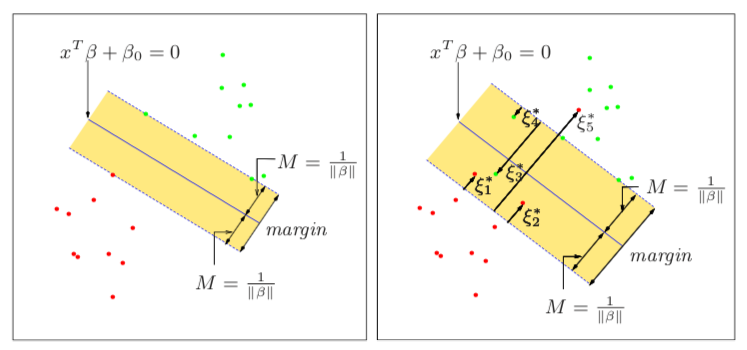
\includegraphics[scale=0.5]{img/SVM}
\caption{Separable and non separable support vector classifiers.}
\end{figure}
The misclassified points are on the wrong side for an amount $\xi^* = M \xi$ while the correctly classified points have $\xi^*=0$. One sees that points inside their class boundary do not play a big role in shaping the boundary. This seems like an attractive property, and one that differentiates it from linear discriminant analysis (\autoref{LDA}). In LDA, the decision boundary is determined by the covariance of the class distributions and the positions of the class centroids. Logistic regression is more similar to the support vector classifier in this regard.

\subsubsection{Computing the support vector classifier}

The problem \autoref{SVMOpt} is quadratic with linear inequality constraints, hence it is a convex optimization problem. We describe a quadratic programming solution using Lagrange multipliers. Computationally it is convenient to re-express \autoref{SVMOpt} in the equivalent form:
\begin{equation}
\begin{aligned}
&\min_{\beta, \beta_0} \frac{1}{2}\left|\beta\right|^2 + C\sum_{i=1}^N \xi_i\\
\textit{subject to } &\xi \ge 0, \quad y_i(x_i^T\beta+\beta_0)\ge 1-\xi_i \quad\forall i
\end{aligned}
\end{equation}
where $C$ replaces the constant. The separable case corresponds to $C = \infty$.
\subsubsection{}
\fi

The problem is quadratic with linear inequalities, hence it is still convex. The Lagrange primal function becomes:
\begin{equation}
L_P = \frac{1}{2}\norm{ \vec{w}}^2 + C \sum_{i=1}^N \xi_i - \sum_{i=1}^N \alpha_i \left[y_i\br{
\vec{w} \cdot \vec{x}_i+b}-\br{1-\xi_i}\right] - \sum_{i=1}^N \mu_i \xi_i 
\label{Lp}
\end{equation}
where $\mu_i$ are the Lagrange multipliers for the newly introduced constraint $\xi_i\ge 0$.
We minimize w.r.t. $\vec{w}, b, \xi_i$. The first two have already been calculated in \autoref{SVMLagrDevw} and \autoref{SVMLagrDevb}:
\begin{equation}
\begin{aligned}
\frac{\partial L_P}{\partial \xi_i} = \Rightarrow \alpha_i &= C - \mu_i \quad \forall i\\
\end{aligned}
\end{equation}
Substituting in \autoref{Lp}, we obtain the Lagrangian (Wolfe) dual objective function:
\begin{equation}
\begin{aligned}
L_D &=  \frac{1}{2}\norm{ \vec{w}}^2 + \cancel{C \sum_{i=1}^N \xi_i} - \sum_{i=1}^N \alpha_i \left[y_i\br{
\vec{w} \cdot \vec{x}_i+b} -1\right]+\cancel{\alpha_i\br{\xi_i}} - \cancel{\sum_{i=1}^N \mu_i \xi_i} = \\
&=\frac{1}{2}\sum_{i=1}^N  \alpha_i y_i \vec{x}_i \cdot \sum_{j=1}^N  \alpha_j y_j \vec{x}_j- \sum_{i=1}^N \alpha_i y_i \vec{x}_i\vec{w} \cancel{- b\sum_{i=1}^N \alpha_i y_i}+ \sum_{i=1}^N \alpha_i =\\
&=\frac{1}{2}\sum_{i=1}^N  \alpha_i y_i \vec{x}_i \cdot \sum_{j=1}^N  \alpha_j y_j \vec{x}_j- \sum_{i=1}^N \alpha_i y_i \vec{x}_i\sum_{j=1}^N \alpha_j y_j \vec{x}_j+ \sum_{i=1}^N \alpha_i =\\
&= \sum_{i=1}^N \alpha_i - \frac{1}{2}\sum_{i=1}^N \alpha_i y_i \vec{x}_i\sum_{j=1}^N \alpha_j y_j \vec{x}_j = \sum_{i=1}^N \alpha_i - \frac{1}{2}\sum_{i=1}^N\sum_{j=1}^N \alpha_i y_i \alpha_j y_j\vec{x}_i  \vec{x}_j
\end{aligned}
\label{LagrangeDueal}
\end{equation}
where we used the properties that $\alpha_i, y_i$ are scalar and that $\vec{w}, b$ can be taken out. Notice that $\vec{w}\cdot \vec{w}  = \sum_{i=1}^N \alpha_i y_i \vec{x}_i\cdot\sum_{j=1}^N\alpha_j y_j \vec{x}_j =\sum_{i=1}^N \sum_{j=1}^N \alpha_i y_i \alpha_j y_j  \vec{x}_i\vec{x}_j \ne \sum_{i=1}^N  (\alpha_i y_i)^2 \vec{x}_i\vec{x}_i$. In fact consider for example: $\vec{w} = c_1\vec{x}_1 + c_2\vec{x}_2$ with $\vec{x}_i = \left[x_{1i}, x_{2i}\right]^T$. $\vec{w} = \left[ c_1x_{11}+c_2x_{12}, c_1x_{21}+c_2x_{22} \right]^T$ and $\vec{w}\cdot \vec{w} = (c_1x_{11}+c_2x_{12})^2+(c_1x_{21}+c_2x_{22})^2$, so we are missing some cross-products. The Lagrangian (Wolfe) dual objective function gives a lower bound on the objective function for any feasible point. We maximize $L_D$ subject to $0\le \alpha_i\le C$ and $\sum_{i=1}^N\alpha_iy_i$. In addition to the derivatives, the \textbf{Karush-kuhn-Tucker} conditions include constraints:
\begin{equation}
\begin{aligned}
\alpha_i \left[ y_i\br{\vec{w}\cdot\vec{x}_i+b}-\br{1-\xi_i}\right] &=0\\
\mu_i \xi_i &= 0\\
y_i(\vec{x}_i\vec{w}+b) - (1 - \xi_i) &\ge 0
\end{aligned}
\label{KKT}
\end{equation}
for $i=1,\cdots, N$. These constraints and the ones originating from the derivatives uniquely characterize the primal and dual problem.

From $\vec{w} = \sum_{i=1}^N  \alpha_i y_i \vec{x}_i$, we can see:
\begin{equation}
\hat{\vec{w}} = \sum_{i=1}^N \hat{\alpha}_i y_i \vec{x}
\end{equation}
with $\hat{\alpha}_i \ne 0$ only for those observations $i$ for which the constraints in the last equation of \autoref{KKT} are exactly met. These observations are called \textbf{support vectors}, since $\hat{\vec{w}}$ is represented in terms of them alone. Among these support points, some will lie on the edge of the margin ($\hat{\xi}_i=0$) and hence will be characterized by $0 < \hat{\alpha_i} <C$: the remainder ($\hat{\xi}_i>0$) have $\hat{\alpha}_i=C$. We can see that any of these margin points ($0<\hat{\alpha}_i$, $\hat{\xi}_i = 0$), can be used to solve for $b$, and we typically use an average of all the solutions for numerical stability. Maximizing the dual is a simpler convex quadratic programming problem than the primal and can be solved with standard techniques such (Murray et. al, 1981).

Points on the wrong side of the boundary are support vectors. In addition, points on the correct side of the boundary but close to it (in the margin), are also support vectors. 

Given the solutions $\hat{\vec{w}}, \hat{b}$, the decision function can be written as:
\begin{equation}
\hat{G} (x) = sign \br{\hat{f}(x)}= sign\br{\hat{\vec{w}}\cdot \vec{x}_i+b}
\end{equation}
The tuning parameter of this procedure is the cost parameter $C$. The optimal value for C can be estimated by cross-validation.
\subsection{Support vector machines and Kernels}
We can make the procedure more flexible by enlarging the feature space using basis expansions such as polynomials or splines. Generally linear boundaries in the enlarged space achieve better training-class separation, and translate to nonlinear boundaries in the original space. 

\subsubsection{Computing SVM for classification}
The Lagrange dual function has the form:
\begin{equation}
L_D = \sum_{i=1}^N \alpha_i - \frac{1}{2}\sum_{i=1}^N\sum_{j=1}^N \alpha_i y_i \alpha_j y_j\left\langle  h(x_i), h(x_j)  \right\rangle 
\end{equation}
So $f(x)$ can be written as 
\begin{equation}
f(x) = h(x)\cdot\vec{w} + b = \sum_{i=1}^N \alpha_iy_i \left\langle  h(x), h(x_i)  \right\rangle +b
\end{equation}

As before, given $\alpha_i$, $b$ can be determined by solving $y_i f(x_i) = 1$ for any (or all) $x_i$ for which $0<\alpha_i <C$.
So $h(x0)$ is involved only in terms of its inner product: \textbf{we do not need to specify the transformation but only the knowledge of the kernel function is required}:
\begin{equation}
K(x, x') = \left\langle  h(x), h(x')  \right\rangle
\end{equation}
$K$ should be symmetric positive (semi-) definite.   Possible popular choices are:

\begin{equation}
\begin{aligned}
\textbf{dth-Degree polynomial:} &\quad K(x, x') = \br{1+\left\langle  x,x'  \right\rangle}^d\\
\textbf{Radial basis:} &\quad K(x, x') =e^{-\gamma\left| x-x' \right|^2}\\
\textbf{Neural Network:} &\quad K(x, x') = tanh\br{k_1\left\langle  x,x'  \right\rangle+k_2}\\
\end{aligned}
\end{equation}
\subsection{SVM for Regression}
SVM can be adapted for regression. The linear regression model is in the form
\begin{equation}
f(x) = x^T\be+\be_0
\end{equation}
and then handle non-linear generalizations. To estimate $\be$ we consider minimization of:
\begin{equation}
\begin{aligned}
H(\be, \be_0) &= \sum_{i=1}^NV\br{y_i - f(x_i)}+\frac{\lambda}{2}\left|\be\right|^2\\
V_\epsilon &=\left\{\begin{array}{ll}0 \quad \quad \textit{if}\quad |r|<1 \\ 
 |r|-\epsilon  \quad \quad \textit{otherwise}
\end{array} 
\right.
\end{aligned}
\end{equation}
\begin{figure}
\centering
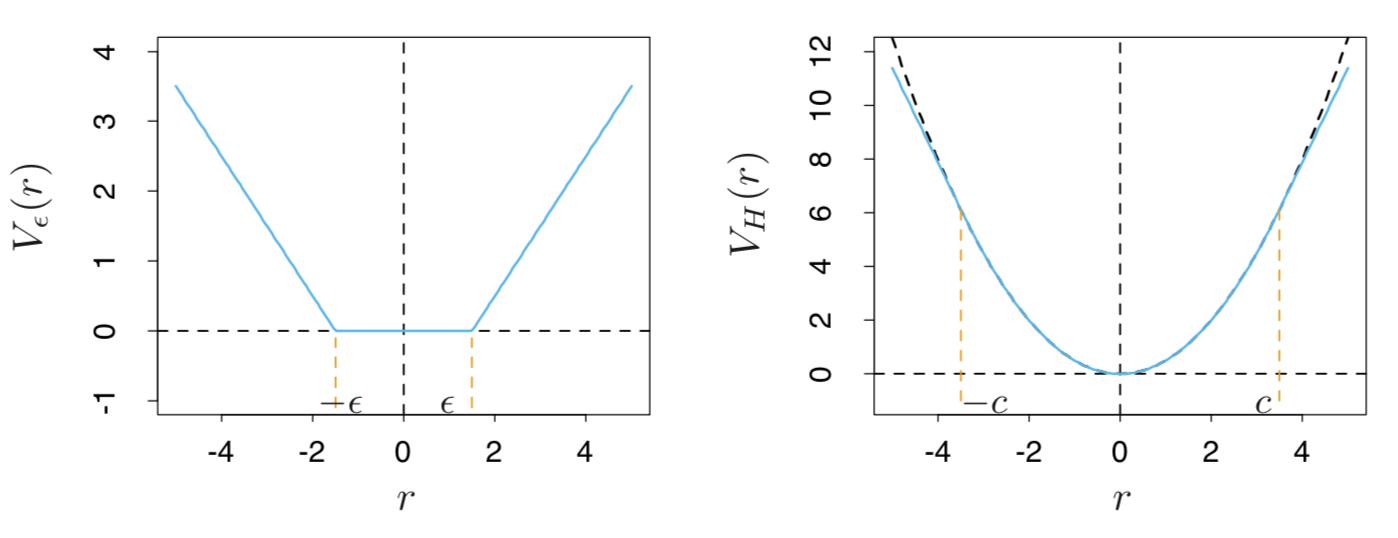
\includegraphics[width=\textwidth]{img/regSVMV}
\caption{The left panel shows the $\epsilon$-insensitive error function used by the support vector regression machine. The right panel shows the error function used in Huber’s robust regression (blue curve) used in statistics. Beyond $|c|$, the function changes from quadratic to linear reducing the contribution of outliers.}
\label{RegSVMV}
\end{figure}
This is an "$\epsilon$-insensitive" error measure, ignoring errors of size less than $\epsilon$ (left panel of \autoref{RegSVMV}). There is a rough analogy with the support vector classification setup, where points on the correct side of the decision boundary and far away from it, are ignored in the optimization. In regression, these "low error" points are the ones with small residuals.

The support vector error measure has linear tails (beyond $\epsilon$), but in addition it flattens the contributions of those cases with small residuals.

If $\be, \be_0$ are the minimizers of $H$, the solution function can be shown to have the form:
\begin{equation}
\begin{aligned}
\hat{\be} &= \sum_{i=1}^N(\hat{\alpha}_i^* - \hat{\alpha}_i)x_i\\
\hat{f}(x) &= \sum_{i=1}^N(\hat{\alpha}_i^* - \hat{\alpha}_i)\left\langle x,x_i\right\rangle+\be_0
\end{aligned}
\end{equation}
where $\hat{\alpha}_i^*, \hat{\alpha}_i$ are positive and solve the quadratic problem:
\begin{equation}
\begin{aligned}
&min_{\alpha_i, \alpha_i^*}\epsilon \sum_{i=1}^N(\alpha_i^* + \alpha_i)-\sum_{i=1}^Ny_i(\alpha_i^* - \alpha_i)+\frac{1}{2}\sum_{i,j=1}^N(\alpha_i^* - \alpha_i)(\alpha_j^* - \alpha_j)\left\langle x_i,x_j\right\rangle\\
&\textit{subject to} \left\{ \begin{array}{lll}
		0 \le \alpha_i, \alpha_i^* \le \frac{1}{\lambda}\\
		\sum_{i=1}^N  (\alpha_i^* - \alpha_i) =0\\
		\alpha_i, \alpha_i^* = 0
		\end{array}
		\right.
\end{aligned}
\end{equation}
Due to the nature of these constraints, typically only a subset of the solution values $(\hat{\alpha}_i^* - \hat{\alpha}_i^*)$ are nonzero, and the associated data values are called the support vectors.
There are two parameters: $\epsilon$ is a parameter of the loss function. $\lambda$ is a regularization parameter and can be estimated by cross validation.

\textbf{The SVM can be extended to multiclass problems} by solving many two-class problems. A classifier is built for each pair of classes and the final classifier is the one that dominates the most.

\subsection{Generalized  LDA}
LDA is a simple prototype classifier which classifies points closest to the centroid. LDA is the estimated Bayes classifier if the observations are multivariate Gaussian in each class, with common covariance matrix, which is very unlikely. LDA has linear boundaries and provides natural low-dimensional views of data. Despite these properties, it fails in a number of situations. One is when more flexibility at for the boundaries is required; in this case QDA works. It does not work well neither with too many correlated predictors, for example in case of digitalized analogue signals and images, since in this case it uses too many parameters. Finally, LDA assumes a single centroid (prototype) per class (and a common covariance matrix) to describe the spread of the data in each class. Sometimes  several centroids are more appropriate.

Three alternatives exist to these three situations:
\begin{itemize}
\item \textbf{recast the LDA problem as a linear regression problem}, which in turn can be converted to a non-parametric form of regression, achieving more flexibility. These are called \textbf{FDA}. The regression procedures can be seen to identify an enlarged set of predictors via basis expansions. FDA amounts to LDA in this enlarged space.
\item When there are too many predictors, we do not want to expand the set. The second idea is to fit LDA but penalize its coefficients to be smooth or otherwise coherent in the spatial domain, such as an image. This is called \textbf{Penalized Discriminant Analysis (PDA)}.
\item \textbf{Model each class by a mixture of two or more Gaussians with different centroids sharing the same covariance matrix}. This allows for more complex decision boundaries and allows for subspace reduction. This is called \textbf{Mixture Discriminant Analysis (MDA)}.
\end{itemize}

\subsubsection{Flexible Discriminant Analysis (FDA)}
This technique performs LDA using linear-regression on derived responses.
Assume we have observations with a quantitative response $G$ falling into one of $K$ classes. Suppose $\theta:\CMcal{G} \rightarrow \CMcal{R}^1$ is a function that assigns scores to the classes such that the transformed class labels are optimally predicted by linear regression, producing the derived responses. Then, having as training examples $(g_i, x_i)$, we solve:
\begin{equation}
\min_{\theta, \be} \sum_{i=1}^N \br{\theta(g_i)-x_i^T\be}^2
\end{equation}
with restrictions on $\theta$ to avoid trivial solutions(mean zero and unit variance over the training data).

More generally, we can find up to $L \le K-1 $ sets of independent scorings for the class labels, $\theta_1, \theta_2, \cdots , \theta_L$, and $L$ corresponding linear maps $\eta_\ell(X) = X^T \be_\ell, l = 1,\cdots, L$, chosen to be optimal for multiple regression in $\CMcal{R}^p$. So the mapping function for one class does not to be the same for the others.

The scores $\theta_\ell(g)$ and maps $\be_\ell$ are chosen to minimize the average squared residual:
\begin{equation}
ASR = \frac{1}{N}\sum_{\ell=1}^N\left[ \br{\theta_\ell(g_i) - x_i^T\be_k}^2\right]
\end{equation}
The set of scores are assumed to be mutually orthogonal and normalized with respect to an appropriate inner product to prevent trivial zero solutions.

The Mahalanobis distance of a test point $x$ to the $k-th$ class centroid $\hat{\mu}_k$ is given by:
\begin{equation}
\delta_j (x, \hat{\mu}_k) = \sum_{\ell=1}^{K-1} w_\ell \br{\hat{\eta}_\ell(x) - \eta_\ell^{-k}(x) }+D(x)
\end{equation}
where $\eta_\ell^{-k}(x) $s is the mean of $\hat{\eta}_\ell(x)$ in the $k-th$ class, and $D(x)$ does not depend on $k$ and $w_\ell$ are defined in terms of the mean squared residual $r_\ell^2$ f the $\ell$th optimally scored fit:
\begin{equation}
w_\ell = \frac{1}{r_\ell^2(1-r_\ell^2}
\end{equation}
To summarize, LDA can be performed by a sequence of linear regressions, followed by classification to the closest class centroid in the space of fits.

The power is that we can replace the linear regression with more flexible non-parametric fits, achieving a more flexible classifier. We can use generalized additive fits, spline functions, MARS and others. In this more general form the regression problems are defined by the criterion:
\begin{equation}
ASR \br{\{\theta_\ell, \eta_\ell \}_{\ell=1}^L} = \frac{1}{N}\sum_{\ell=1}^L\left[\sum_{i=1}^N \br{\theta_\ell(g_i) - \eta_\ell(x_i)}^2 + \lambda J(\eta_\ell)\right]
\end{equation}
where $J$ is a regularizer appropriate for some forms of nonparametric regression.

The computations of FDA coordinates can be simplified in cases when the nonparametric procedure can be represented as a linear operator $\mathbf{S}_\lambda$, that is $\hat{\y} =\mathbf{S}_\lambda \y$. Additive splines have this property if the smoothing parameters are fixed, as well as MARS when the basis functions are selected. The subscript $\lambda$ denotes the entire set of smoothing parameters. If $\mathbf{S}_\lambda = \mathbf{H}_X$, the linear regression projection operator, then we are back to LDA.

We create $N \times K$ \textit{indicator response matrix} \textbf{Y} from the response $g_i$, such that $y_{ik} = 1$ if $g_i =k$, $0$ otherwise. Each row in $\mathbb{Y}$ has only one $1$.
The steps are the following:
\begin{enumerate}
\item \textbf{Multivariate nonparametric regression}: fit a multiresponse, adaptive nonparametric regression of $\mathbf{Y}$ on $\mathbf{X}$, giving the fitted values $\mathbf{\hat{Y}}$. Let $\mathbf{S}_\lambda$ be the linear operator that fits the final chosen model and $\eta^*(x)$ be the vector of fitted regression functions \label{MNR}.
\item \textbf{Optimal scores}: compute the eigen-decomposition of $\mathbf{Y}^T\mathbf{\hat{Y}}=\mathbf{Y}^T\mathbf{S}_\lambda \mathbf{Y}$ where the eigenvectors $\mathbf{\Phi}$ are normalized: $\mathbf{\Phi}^T\mathbf{D}_\pi\mathbf{\Phi}^T$. here $\mathbf{D}_\pi = \mathbf{Y}^T\mathbf{Y}/N$ is a diagonal matrix of the estimated class prior probabilities.
\item \textbf{Update} the model from step \autoref{MNR} using the optimal scores $\eta(x) = \Phi^T\eta^*(x)$.
\end{enumerate}  
\subsubsection{Penalized discriminant analysis}
Although FDA is motivated by generalizing optimal scoring, it can also be viewed directly as a form of regularized discriminant analysis. Suppose the regression procedure used in FDA amounts to a linear regression onto a basis expansion $h(X)$, with a quadratic penalty on the coefficients:
\begin{equation}
ASR\br{\{ \theta_\ell, \be_\ell\}_{\ell=1}^L} = \frac{1}{N}\sum_{\ell=1}^L\left[\sum_{i=1}^N \br{\theta_\ell(g_i) - h^T(x_i)\be_\ell}^2 + \lambda \be_\ell^T\Omega \be_\ell\right]
\end{equation}
The choice of $\Omega$ depends on the problem. if $\eta_\ell(x) = h(x)\be_\ell$ is an expansion on spline basis functions, $\Omega$ might constrain $\eta_\ell$ to be smooth over $\CMcal{R}^p$. In the case of additive splines, there are $N$ spline basis functions for each coordinate, resulting in a total of $N_p$ basis functions in $h(x)$; $\Omega$ in this case is $N_p \times N_p$ and block diagonal.

The steps in FDA can then be viewed as a generalized form of LDA, which we call penalized discriminant analysis, or PDA:
\begin{itemize}
\item Enlarge the set of predictors $X$ via a basis expansion $h(X)$.
\item Use (penalized) LDA in the enlarged space where the Mahalanobis distance is given by:
\begin{equation}
D(x, \mu) = \br{h(x) - h(\mu)}^T\br{\Sigma_W+\lambda\Sigma}^{-1} \br{h(x) - h(\mu)}
\end{equation}
where $\Sigma_W$ is the within-class covariance matrix of the derived varaibles $h(x_i)$.
\item Decompose the classification subspace using a penalized metric:
\begin{equation}
\max u^t\Sigma_{Bet}u \quad\quad \textit{subject to} \quad u^T\br{\Sigma_W+\lambda\Sigma}u =1
\end{equation}
\end{itemize}
For some classes of problems, the first step, involving the basis expansion, is not needed; we already have far too many (correlated) predictors. An example is when the objects are digitalized analogue signals. Neighbouring pixel values will tend to be correlated, being often almost the same. This implies that the pair of corresponding LDA coefficients for these pixels can be wildly different and opposite in sign, and thus cancel when applied to similar pixel values. Positively correlated predictors lead to noisy, negatively correlated coefficient estimates, and this noise results in unwanted sampling variance. A reasonable strategy is to regularize the coefficients to be smooth over the spatial domain, as with images. This is what PDA does. The computations proceed just as for FDA, except that an appropriate penalized regression method is used.

\subsubsection{Mixture Discriminant Analysis}
Linear discriminant analysis can be viewed as a prototype classifier. Each class is represented by its centroid, and we classify to the closest using an appropriate metric. In many situations a single prototype is not sufficient to represent inhomogeneous classes and mixture models are more appropriate.

A Gaussian mixture model for the $k-th$ class has density:
\begin{equation}
P(X|G=k) = \sum_{r=1}^{R_k} \pi_{kr}\phi(X, \mu_{kr},\Sigma)
\end{equation}
where the \textbf{mixing proportions}$\pi_{kr}$ sum to one. The class posterior probabilities are given by
\begin{equation}
P(G=k|X=x) = \frac{\sum_{r=1}^{R_k} \pi_{kr}\phi(X, \mu_{kr},\Sigma)\Pi_k}{\sum_{\ell=1}^K\sum_{r=1}^{R_\ell} \pi_{\ell r}\phi(X, \mu_{\ell r},\Sigma)\Pi_\ell}
\end{equation}
where $Pi_k$ are the class priors.

As in LDA we estimate the parameters by MLE, using the joint log-likelihood based on $P(G,X)$:
\begin{equation}
\sum_{k=1}^K\sum_{g_i=k} \log \left[ \sum_{r=1}^{R_k} \pi_{k r} \phi (x_i,\mu_{k r}, \Sigma)\Pi_k\right]
\end{equation}
The sum within the log makes this a rather messy optimization problem if tackled directly. The classical and natural method for computing the maximum-likelihood estimates (MLEs) for mixture distributions is the EM algorithm. EM alternates between the two steps:
\begin{itemize}
\item \textbf{E-step} Given the current parameters, compute the \textbf{responsability} of subclass $c_{kr}$ within class $k$ for each of the class-$k$ observations ($g_i=k$):
\begin{equation}
W(c_{kr}|x_i, g_i) = \frac{ \pi_{kr}\phi(x_i, \mu_{kr},\Sigma)}{\sum_{\ell=1}^{R_k} \pi_{k \ell}\phi(x_i, \mu_{k \ell},\Sigma)}
\end{equation}
\item \textbf{M-step}: compute the weighted MLEs for the parameters of each of the component Gaussians within each of the classes, using the weights from the E-step.
\end{itemize}

In the E-step, the algorithm apportions the unit weight of an observation in class k to the various subclasses assigned to that class. If it is close to the centroid of a particular subclass, and far from the others, it will receive a mass close to one for that subclass. On the other hand, observations halfway between two subclasses will get approximately equal weight for both.

In the M-step, an observation in class k is used $R_k$ times, to estimate the parameters in each of the $R_k$ component densities, with a different weight for each.